\documentclass[a4paper,11pt]{book}
\usepackage[spanish,es-tabla]{babel} %Indica que escribiermos en español
% Incluir imágenes en LaTeX
\usepackage{csquotes}
\usepackage[usenames]{color} % Para colorear texto
\usepackage{subfigure} % subfiguras
\usepackage{booktabs}
\usepackage[table]{xcolor}
\usepackage{sidecap} % Para poner el texto de las imágenes al lado
	\sidecaptionvpos{figure}{c} % Para que el texto se alinie al centro vertical
\usepackage{caption} % Para poder quitar numeracion de figuras
\usepackage{pdfpages}
\usepackage{graphicx, amsmath, amsthm, latexsym, amssymb, amsfonts, epsfig, float, enumerate, color, listings,  graphicx, fancyhdr}
\usepackage{flushend}
\usepackage{appendix}
\usepackage{pdfpages}
\usepackage{parskip}
\usepackage{float}
\usepackage{amsmath, amsthm, amssymb, amsfonts}
\usepackage[hidelinks]{hyperref}%para meter lins con \href

\usepackage{anysize} 					% Para personalizar el ancho de  los márgenes
\hypersetup{
    colorlinks=true,
    linkcolor=black,
    filecolor=magenta,      
    urlcolor=cyan,
}%para colores de links
\date{}

\providecommand{\abs}[1]{\lvert#1\rvert}
\providecommand{\norm}[1]{\lVert#1\rVert} %comandos para poder poner en valor absoluto funciones o valores.
\usepackage{multicol}%paquete para crear multicolumna
\setlength\columnsep{18pt}%Especifíca separación de las columnas
\marginsize{2cm}{2cm}{1.25cm}{2cm} % Izquierda, derecha, arriba, abajo
\usepackage{flushend}
\usepackage{appendix}
\usepackage{pdfpages}
\usepackage{parskip}
\usepackage{float}
\usepackage{subfigure}

\date{}
\usepackage[maxbibnames=99, sorting=none]{biblatex}
\usepackage{fancyhdr}
\fancyhf{}
\fancypagestyle{plain}{
    \setlength{\headheight}{14pt}
}%esto pone el encabezado arriba derecha con la raya
\fancyhf{}
	\fancyfoot[C]{\thepage}
\renewcommand{\headrulewidth}{0.5pt}
\pagestyle{fancy}
%copiar esto para poner encabezado con linea, sobra algo pero no se el que.
\pagestyle{plain}
\renewcommand{\tablename}{Tabla}
\def\tablename{Tabla}
\graphicspath{{./img/}}

\begin{document}


%%%%%%%%%%%%%%%%%%%%%%%%%%%%%%%%%% PORTADA %%%%%%%%%%%%%%%%%%%%%%%%%%%%%%%%%%%%%%%%%%%%
																					%%%
\begin{center}																		%%%
\newcommand{\HRule}{\rule{\linewidth}{0.5mm}}									%%%
	\vspace{0.5\textheight}

    \begin{center}
        \Huge{\textbf{Apuntes sobre la bibliografía}}

    \end{center}
\end{center}
\chapter{Percolation theory of self-exciting temporal processes}

En este artículo se tratan las propiedades de patrones de actividad inhomogéneos que aparecen en la vida real. Estos dependen de la resolución temporal que 
utilicemos para definir las ráfagas o avalanchas de actividad. En el artículo se encuentra que el mismo proceso puede dar lugar a diferentes duraciones 
y tamaños de estas avalanchas, cosa que achacan a la ``competición'' entre la percolación en 1D (tiempo) y una universalidad en los procesos de ramificación
(estados accesibles en cada tiempo). Se observa que hay regimes causados putamente por esta universalidad para valores específicos del parámetro de 
resolución, que además coinciden con los puntos críticos en el diagrama de percolación.

Nosotros estamos interesados en estudiar este tipo de fenómenos ya que en el cerebro ocurren estos patrones inhomogéneos de actividad. Además de la 
característica de ser en ráfagas, tanto la duración como la intensidad de estas tienen una distribución de leyes de potencias.

Si el fenómeno a estudiar consiste en eventos puntuales (discretos) en el tiempo, tanto el tamaño como la duración de las ráfagas se obtienen del tiempo 
entre dichos eventos. Además, se demuestra que este tiempo entre eventos sigue una distribución \textit{fat-tailed}. En este tipo de series temporales, 
las avalanchas relacionadas con actividad son monitorizadas haciendo más gruesa la serie temporal para una escala de tiempo fija. Las correlaciones las podemos 
medir asignando eventos a una misma ráfaga siempre que el tiempo entre eventos sea menor que un umbral determinado. Este umbral lo podemos escoger arbitrariamente
o se puede imponer dependiendo de la resolución temporal de los datos experimentales. 

A lo largo del artículo intentaremos entender la relación entre la resolución temporal y las estadística de las ráfagas. Para ello, vamos a introducir una 
técnica que nos permite determinar la resolución temporal que se debería usar para definir las avalancas de una serie temporal. Validaremos este método en 
series temporales que siguen procesos de Hawkes, modelos de comportamiento autocorrelecionado para la descripción de terremotos y \textbf{redes neuronales}.
El uso de estos procesos de Hawkes nos permitirá controlar completamente el mecanismo que genera las correlaciones\footnote{Esto es debido a que nos permite 
controlar la intensidad de los procesos $\mu$ como veremos después.} además de la posibilidad de abarcar el problema de manera analítica.

Primero comenzamos definiendo un grupo de actividad de manera consistente con una avalancha causada por eventos muy cercanos. Los datos están representados 
por $K$ eventos $\left\{ t_1,\ldots,t_K \right\}$, donde $t_i$ es el tiempo de ``aparición'' del evento i-ésimo. Sea $\Delta\geq0$ el parámetro de resolución 
fijo para identificar los grupos de actividad. Supongamos que un grupo empieza en un tiempo $t_b$ está compuesto por $S$ eventos consecutivos 
$\left\{ t_b,t_{b+1},\ldots t_{b+S-1} \right\}$ tal que $tn-t_b-1>\Delta$, $t_{b+s}-t_{b+S-1}\Delta$ y $t_{b+i}-t_{b+i-1}<\Delta$ para todos los eventos. 
Es decir que los eventos de la avalancha difieren temporalmente menor al parámetro de resolución. Asumimos también que $t_0=-\inf$ y $t_{K+1}=+\inf$, cosa que
implica que el primer y último evento empiezan y acaban respectivamente un grupo. Definimos el tamaño $S$ como el número de eventos dentro del grupo y su duración
como $T=t_{b+S-1}-t_b$, es decir, el tiempo entre el primer y último evento del grupo.

Si el parámetro de resolución $\Delta$ es más grande que el mayor tiempo entre eventos, entonces solo tenemos un grupo de tamaño $K$ y duración $t_K-t_1$. 
Por otro lado, si $\Delta$ es menor que el menor tiempo entre eventos, cada evento forma un grupo de tamaño 1 y duración 0. Como en la mayoría de problemas de 
percolaciones unidimensionales, esperamos un valor intermedio $\Delta=\Delta^*$ que haga que pasemos de una fase en la que no hay percolaciones a una en la 
que sí que hay. Por lo que es interesante preguntarnos, ¿qué podemos sacar del diagrama de percolaciones de la serie temporal? ¿Fijar la resolución temporal
$\Delta=\Delta^*$ nos permite observar propiedades del proceso que no serían visibles en otro caso?

Para obtener la ``configuración controlada'' vamos a generar las series temporales via procesos de Hawkes con un \textit{rate} condicional:
\begin{equation}
    \lambda(t|t_1,\ldots,t_k) = \mu+ n\sum_{i=1}^{k}\phi(t-t_i).
    \label{eq:eq1}
\end{equation}

Es decir, el \textit{rate} depende de los $k$ eventos pasados. El primer término de la ecuación produce eventos espontáneos cuando $\mu\geq0$. El 
segundo término es la suma de las contribuciones individuales de los eventos anteriores. Debemos tener en cuenta que la función $\phi(x)$ es la 
llamada función de excitación o función kernel del proceso de autoexcitación, suponemos que es no negativa y es monótonamente no creciente. Funciones típicas 
de este tpo son exponenciales o leyes de potencia decrecientes, estudiaremos los dos casos. Por otra parte, en la ecuación \ref{eq:eq1} asumiremos que 
$$\int_{0}^{\infty}\phi(x)dx=1$$
de esta forma, el término de la memoria estará ``dentro'' solo del parámetro $n\geq0$. A no ser que digamos otra cosa, siempre tomaremos $n=1$, que 
corresponde al regimen crítico de la dinámica del proceso descrito por la ecuación (se demuestra en una referencia).

El marco de percolación nos permite caracterizar el proceso genérico de Hawkes de la ecuación \ref{eq:eq1} utilizando análisis de escala de tamaño finito.
El número total de eventos $K$ en la serie temporal será el tamaño del sistema. Para un $K$ dado, generaremos múltiples series temporales y calcularemos 
la fuerza de percolación $P_{inf}$, es decir, la fracción de eventos pertenecientes al grupo (\textit{cluster}) más grande, además calcularemos 
también la susceptibilidad asociada. Estudiando el comportamiento de estos parámetros para valores de $K$ crecientos, podremos estimar el valor de los 
umbrales y de los exponentes críticos.

Comenzamos con el caso $n=0$, el cual que describe un proceso de Poisson homogéneo de \textit{rate} $\mu$. El tiempo entre eventos será $x_i=t_i-t_{i-1}$
y estará distribuido como una distribución de Poisson $=(x_i)=\mu e^{-\mu x_i}$. Por lo tanto, dos eventos consecutivos serán parte del mismo grupo con 
una probabilidad $P(x_i \leq \Delta)=1-e^{\mu\Delta}$, que es independiente al índice. Para valores de $K$ finitos, $P_{\inf}$ crece muy picádamente de 0 
a 1 entorno al punto pesudocrítico $\Delta^*(K)=log(K)/\mu$. Por otro lado, podemos comprobar que las distribuciones del tamaño del grupo $P(S)$ y la 
duración $P(T)$ están descritos exáctamente por la teoría de percolaciones unidimensionales (se demuestra en otra ref). Estos son el producto de una ley 
de potencias escalada con una función que decrece muy rápido y que depende el tamaño del sistema. En este caso, las funciones de escala contienen un 
término multiplicando que exáctamente la ley de pontencias, por lo tanto, la distribución tiene un comportamiento exponencial en $\Delta=\Delta^*$.
Además, se puede comprobar la criticidad en la relación entre el tamaño y la duración $\langle S\rangle\sim T$, que concuerda con la relación 
$\langle S\rangle\sim T^{(\alpha-1)/(\tau-1)}$.

Ahora vamos a considerar los procesos de Hawkes con un \textit{kernel} exponencial $\phi(x)=e^-x$. Los resultados para $\mu\ll1$ y $\gg1$ junto con los 
ya mencionados se ven en la figura \ref{f:fig1}

\begin{figure}[H]
\centering
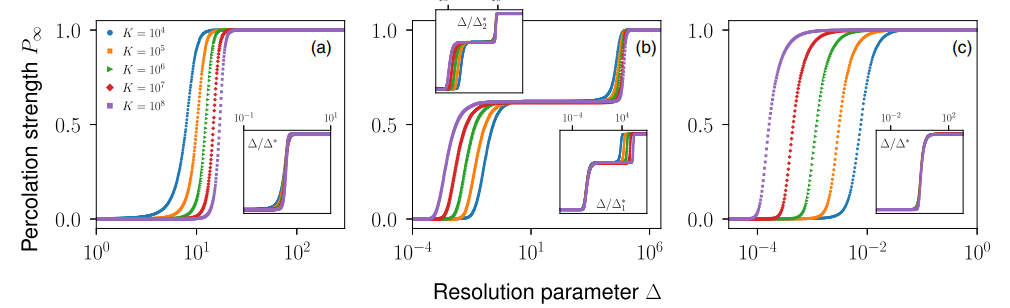
\includegraphics[width=0.9\textwidth]{fig1.PNG}   
\caption{Diagramas de percolación de procesos de autoexcitación.}
\label{f:fig1} 
\end{figure}

Para $\mu\ll1$ encontramos mucha fenomenolgía, con dos transiciones distintas en $\Delta^*_1<\Delta^*_2$ respectivamente. Entorno al punto $\Delta^*_1$, 
el sistema está caracterizado por un comportamiento compatible con la universalidad de las percolaciones unidimensionales, es decir, igual que el caso 
del proceso homogéneo de Poisson. Tanto $P(S)$ como $P(T)$ son leyes de potencias que decaen en $\Delta^*_1$ con exponentes $\tau=\alpha=2$, además 
el tamaño medio y la duración de los grupos están correlacionados linealmente como vemos en la figura \ref{f:f2}.

\begin{figure}[H]
    \centering
    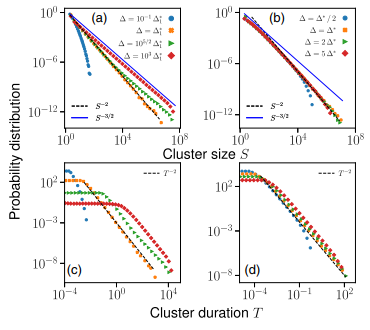
\includegraphics[width=0.6\textwidth]{fig2.PNG}   
    \caption{Propiedades críticas de procesos de autoexcitación temporal con un \textit{kernel} exponencial, $n=1$, un tamaño del sistema de $K=10^8$. Las 
    probabilidades se han obtenido considerando $C=10^7$ grupos por configuración.}
    \label{f:f2} 
\end{figure}

El umbral pesudocrítico se da en $\Delta^*_1\simeq log(K)/\langle \lambda\rangle=log(K)/(\mu+\sqrt{2K\mu})$. Donde $\langle \lambda\rangle$ es el valor 
esperado del \textit{rate} de que se hayan dado $K$ eventos sobre un número infinito de realizaciones del proceso. La otra transicón se da en 
$\Delta^*_2= log(K)/\mu$, que tiende a infinito cuando crece $K$. Esta corresponde a una fusión de toda la serie temporal en un solo grupo, sus características
son compatibles con las de la universalidad un proceso de ramificación de campo medio, es decir $\tau=3/2$ y $\alpha=2$.


Para $\mu\gg1$ el diagrama de fase solo tiene un cambio de fase, con características idénticas a la de $\mu\ll1$, además, los exponentes son los 
mismos $\tau=\alpha=2$. Los dos comportamientos diferentes observados para $\mu\gg1$ y $\mu\ll1$ se interpretan en un mismo marco. Para $\mu\ll1$
el proceso está caracterizado por una secuencia de ráfagas autoexcitadas debidas al término de memoria de la ecuación \ref{eq:eq1}. Esta memoria 
decae exponencialmente muy rápido, con una escala temporal típicamente de la unidad. Cada ráfaga es un evento espontáneo caracterizado por la 
escala temporal $1/\mu\gg1$, por lo que las ráfagas están bien separadas entre sí. Al aumentar $\Delta$, el sistema tiene una primera transición 
entre ráfagas en $\Delta=\Delta^*_1$ correspondiente a la fusión de eventos de la mmisma ráfaga, y posteriormente una transición a través
de ráfagas en $\Delta^*_2$ correspondiente a la fusión de ráfagas de actividad consecutivas. 

Para $\mu\gg1$, todos los eventos pertenecen a una sola ráfaga de autoexcitación. En este caso, la escala de tiempo de la actividad espontánea es 
igual o menor que la de autoexcitación. Aun así, aunque la memoria decae exponencialmente rápico, un evento espontáneo reexcita el proceso lo 
suficientemente rápico para que la ráfaga prosiga. Debemos tener en cuenta que la ráfaga está truncada en las simulaciones debido al tamaño fijo 
$K$ de las series temporales. Cuando la resolución $\Delta$ aumenta, todos los eventos de una sola ráfaga se fusionan en un solo grupo y por tanto,
la transición es del mismo tipo que en las ráfagas en $\Delta=\Delta^*_1$ cuando $\mu\ll1$.

Para finalizar, simplificaremos el proceso dando $\mu=0$ y asumiendo que el primero evento de la ráfaga ya ha ocurrido. Después de esto, ``invocamos'' 
el mapa conocido de procesos de autoexcitación de nuestra ecuación de los procesos de ramificación de Galton Walton. de acuerdo con estos, el primer 
evento de la serie representa la raíz de un árbol que se ramidica, cada evento genera un número de ``descendencias'' siguiendo una distirbución de 
Poisson con valor medio $n$, el parámetro de la ecuación \ref{eq:eq1}. Supongamos que el primer evento ocurre en $t_1$ que suponemos que es $0$ por 
simplicidad. De esta forma, cada uno de los eventos siguientes tiene un tiempo asociado igual al tiempo de su padre mas un valor aleatorio $x$ extraído 
por la función \textit{kernel} $\phi(x)$. Mapear este proceso nos ofrece una manera alternativa (en media es estadísticamente equivalente) de 
generar series temporales que sigan nuestra ecuación.

Primero generamos el árbol, después asociamos un tiempo a cada evento siguiendo las reglas establecidas anteriormente. El tiempo $t$ asociado 
a un evento de la generación g-ésima se distribuirá como la función $P(t\Big|g)$. Para el caso del \textit{kernel} exponencial, esta es la 
suma de las $g$ variables distribuidas exponencialmente, es decir, la distribución de Erlang de \textit{rate} igual a 1:
$$P(t|g)=\dfrac{t^{g-1}e^{-t}}{(g-1)!}$$

Además, el mapeado de los procesos de autoexcitación como procesos de ramificación nos permite entender las valores numéricos obtenidos en las 
figuras \ref{f:fig1} y \ref{f:f2}. Para $n=1$ el proceso de ramificación es crítico. La distribución del tamaño del árbol sogue $P(Z)\sim Z^{-3/2}$ 
y la distribución de la profundidad de este (tiempo) $P(D)\sim D^{-2}$. Como hemos visto, ráfagas individuales de actividad para valores altos de 
resolución $\Delta$ y $\mu\ll1$ siguene stas estadísticas. en concreto, el tamaño de cada ráfaga $S$ es exáctamente el tamaño $Z$ del árbol. Y la 
media de la duración de las ráfagas sigue $\langle T\rangle\sim D$ como esperábamos.

Para el espacio entre los dos umbrales $\Delta\in\left[ \Delta^*_1,\Delta^*_2 \right]$, $P_{\inf}$ de la figura \ref{f:fig1}(b) sigue la misma estadística 
que el máximo de una muestra de variables extraídas de la distribución $P(Z)\sim Z^{-3/2}$ dividida por su suma.

Por otro lado, el comportamiento cuando $\Delta=\Delta^*_1$ y el \textit{crossover} del régimen de los procesos de ramificación para valores grande de 
resolución se deben debido a fenómenos de umbral. Esto sigue la naturaleza de la percolación en procesos de Poisson. Dado un árbol de ramificación 
${n_1,N_2,\ldots N_g,\ldots,N_G}$ donde $N_g$ indica el número de eventos de la g-ésima generación del árbol, la serie temporal del proceso de 
Hawkes es estadísticamente equivalente a un proceso de Poisson inhomogéneos con \textit{rate} $\hat{\lambda}(t|N_1,\ldots,N_G)=\sum_gP(t|g)N_g$.
Por lo tanto, dada una resolución $\Delta$, siempre que $\bar{\lambda}(t|N_1,\ldots,N_G)<1/\Delta$, los eventos entorno al tiempo t 
pertenecerán a grupos diferentes y por lo tanto, el número total de eventos $S_T$ que forman un grupo de actividades conduración $T$ es la integral de 
la curva de $\hat{\lambda}(t|N_1,\ldots,N_G)$ a lo largo del tiempo en el que el \textit{rate} es mayor que $\Delta^{-1}$. Esta integral se puede 
dividir en dos contribuciones, una correspondiente a área del orden de $T^2$ que aparece sobre la línea del umbral de la figura \ref{f:fig3} y otra 
correspondiente al área $\Delta^{-1}T$ que aparece debajo del umbral.
\begin{equation}
    S_T\sim T^2+\Delta^{-1}T
    \label{eq:eq2}
\end{equation}

Mientras que la distribución del grupo es siempre la misma (es decir, $P(T)\sim T^{-2}$), si $\Delta^{-1}>T$, entonces, $S_T\sim T$, lo que implica 
que estamos en la estadística de dentro de la ráfaga. Si $\Delta^{-1}<T$, entonces $S_\sim T^2$ y la conservación de la probabilidad da lugar a la estadística 
de procesos de ramificación $P(S)\sim S^{-3/2}$. Como resumen, podemos obtener una comprensión completa del tamaño $(P(S))$ observando que el escalado de 
la ley de potencias requiere que se observe un tamaño de muestra mínimo, suficiente para que el grupo más grande tenga una duración comparable a $\Delta^{-1}$.
si la muestra no es lo suficientemente grande, la distribución será exponencial (se demuestra en otra referencia).


Finalmente, si consideramos una ley de potencias en el \textit{kernel}:
$$\phi=(\gamma-1)(1+x)^{-\gamma}$$

nos damos cuenta que la estructura de ramificación del proceso no se ve afectada, por lo que los resultados deberian ser los mismos. Por otro lado, 
para $\gamma>2$ $\phi(x)$ tiene valor medio finito, y por lo tanto, los resultados son los mismos que con el \textit{kernel} exponencial. En concreto, 
$P_{\inf}$ tiene una transición de discontínua cuando $\mu\gg1$ mientras que tiene dos transiciones para $\mu\ll1$. La distribucióndel tamaño del grupo 
tiene un cruce entre $\tau=2$ en $\Delta^*_1$ a $\tau=3/2$ para $\Delta\gg\Delta_1^*$ cuando $\mu\ll1$, por otro lado, el exponente $\tau=2$ no 
tiene ningún cruce cuando $\mu\gg1$. 

En el caso $\gamma\leq2$, $\phi(x)$ no tiene definido el valor medio, y el tiempo típico entre evento es tan largo que no podemos aplicar este ``modelo''.


\begin{figure}[H]
    \centering
    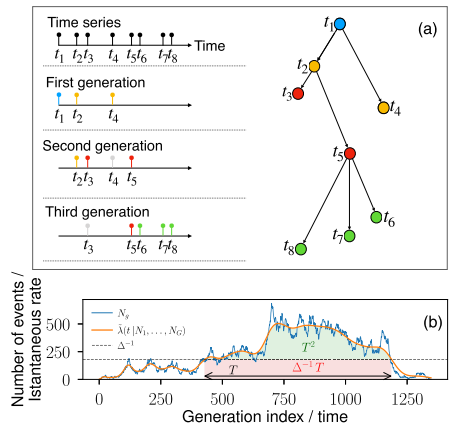
\includegraphics[width=0.6\textwidth]{fig3.PNG}   
    \caption{Estructura de árbol en procesos de autoexcitación.}
    \label{f:fig3} 
\end{figure}

\chapter{Ubiquitous Power Law Scaling in Nonlinear Self-Excited Hawkes Processes}

De este artículo nos interesa en principio solo la introducción y poco más en principio.

El artículo comienza comentando que encontramos muchas funciones de distribución con colas (\textit{power law tails}) en muchos campos de la ciencia como las 
ciencias lingüísticas, sociales, naturales... Paralelamente, comentan que también encontramos muchos procesos cuya dinámica es de autoexcitación, desde la 
física del ruido, hasta los procesos sísmicos. Motivados por los procesos de activación de la forma de Arrhenius, el artículo une estos dos hilos introduciendo
una clase de procesos autoexcitados no lineales con intensidades de rápida aceleración en función de un parámetro que llamaremos ``tensión''. Al resolver 
las ecuaciones maestras correspondientes, encontramos que una amplia clase de procesos de Hawkes no lineales tienen una función de distribución de probabilidad 
descrita por una ley de potencias con las condiciones de que (i) la intensidad sea una función de la tensión que se acelera rápidamente, (ii) la 
distribución es bilateral ($\int_{-\infty}^{0}\rho(y)dy\neq0$, $\int_{0}^{\infty}\rho(y)dy\neq0$) con media no positiva ($m:=\int_{-\infty}^{\infty}y\rho(y)dy\leq0$)
y (iii) tiene \textit{fast-decaying tails} ($\Phi(x):=\int_{-\infty}^{\infty}dy\rho(y)(e^{xy}-1)$ existe, tiene dos raíces, una es $0$ y otra $c^*\geq0$). 
En particular, el escalado de Zipf se obtiene en el 
límite donde esta marca promedio desaparede. Esto da lugar a un mecanismo que proporciona distribuciones de leyes de potencia.

\section{Introducción}

Como hemos comentado, muchos tipos de datos dan lugar a distribuciones de ley de potencias para las frecuencias de sus variables características. Es decir, 
la función de densidad de probabilidad (PDF) P(S) de la variable S viene dada por $P(S)\sim1/S^{\alpha+1}$ con $\alpha > 0$. Muchos mecanismos se han propuesto
para describir esto, como el crecimiento proporcional a diferentes condiciones por ejemplo.

Los procesos de autoexcitación asumen que los eventos pasados tienen una gran influencia en los eventos futuros. Los procesos de Hawkes son los más simples 
de este tipo, donde la intensidad (probabilidad por unidad de tiempo de que un nuevo evento ocurra) es lineal en la suma para la influencia de los eventos 
pasados. Además, hemos encontrado en la última década generalizaciones de este tipo de procesos en gran cantidad de campos del conocimiento. Es por este auge 
que aunque sean teóricamente desafiantes, estos procesos se han estudiado profundamente en la mayoría de casos, incluso aunque a priori los procesos 
sean más adecuados para representar la relación entre la stocasticidad y no linealidad de muchos sistemas complejos. En concreto, en este artículo se estudian 
los procesos de Hawkes caracterizados por intensidades de rápida aceleración como función de una variable auxiliar que llamamos tensión y además vemos que 
se puede aplicar a muchos tipos de procesos. Encuentran también que esta familia de procesos de Hawkes tienen intensidades que siguen leyes de potencias. En 
concreto, aparece naturalmente el escalado de Zipf cuando las distribuciones de marcas son simétricas. Una condición más leve es que la media decrece. 

\section{Modelo}

Los ingredientes principales de los procesos de autoexcitación de Hawkes son la intensidad $\lambda(t)$ y la tensión $\nu(t)$. Sea una serie temporal ${t_i}_i$
que representa el tiempo entre eventos, como por ejemplo los terremotos, los retweets en Twitter o las \textbf{descargas neuronales en el cerebro}.
La intensidad $\lambda(t)$ caracteriza completamente la estadística de los eventos, de tal forma que un evento ocurrirá con probabilidad $\lambda(t)dt$ en 
el intervalo $[t,t+dt)$. Asumimos que la intensidad es una función no lineal positiva y monótamente creciente en función de la tensión del sistema:

\begin{equation}
    \lambda(t)=g[\nu(t)]
    \label{eq:lambda de t}
\end{equation}


donde $g(\nu)$ es el mapa de tensión-intensidad y esta tensión cuantifica la influencia de los eventos históricos. Esta tensión en un tiempo dado la podemos 
calcular como una suma de perturbaciones sobre los eventos pasados; 
\begin{equation}
    \nu(t)=\sum_{i=1}^{N(t)}y_ih(t-t_i)
    \label{eq:nu de t}
\end{equation}
donde cada evento $i$ tiene una marca $y_i$ distribuida siguiendo la función de densidad de probabilidad $\rho(y)$ y $N(t)$ es el número de eventos en $[0,t)$.
Combinando esta relación entre entre la tensión y la intensidad nos da lugar a los procesos de Hawkes no lineales.
$$\lambda(t)=g\left[ \sum_{i=1}^{N(t)} y_ih(t-t_i)\right]$$
Para representar que esta alta tensión da lugar a eventos futuros, asumimos que el mapa de intensidad es una función no decreciente. Para una función 
$g(\nu)=\nu_0+\nu$, el modelo con la ecuación \ref{eq:lambda de t} y \ref{eq:nu de t} se reduce a los procesos de Hawkes e $y_i$ puede ser interpretado como 
el número medio de eventos de la primera generación activados por el evento $i$, por lo tanto lo llamaremos evento de fertilidad del evento $i$ imponiendo 
$$\int_{0}^{\infty}h(t)dt=1$$
La función de memoria $h(t)\geq$ controla la distribución en tiempo de los eventos y decaimientos a 0 para valores grandes de $t$.

Todo esto, da lugar a las siguientes gráficas de la tensión, intensidad y densidad de probabilidad que aparecen en la figura \ref{f:f4}

\begin{figure}[H]
\centering
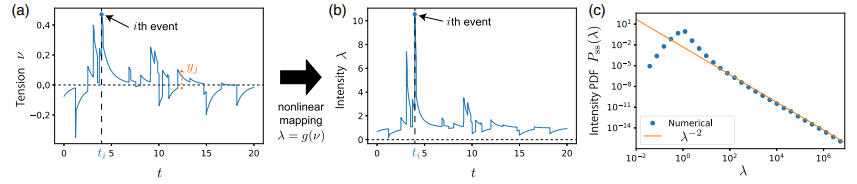
\includegraphics[width=\textwidth]{fig4.PNG}
\caption{Trayectorias de la tensión e intensidad con su respectiva densidad de probabilidad.}
\label{f:f4}    
\end{figure}

\chapter{Exact simulation of Hawkes processwith exponentially decaying intensity}
En el artículo nos dan un algoritmo eficiente para la simulación de porcesos de Hawkes con un kernel exponencial decreciente para el \textit{rate} (intensidad).
Este método es capaz de generar de manera exacta los procesos de Hawkes. Para ello, samplea los tiempos entre eventos directamente con una distribución 
analítica sin necesidad de usar la transformada inversa, por lo que evita la discretización. Además, es flexible en cuanto a ser capaz de generar puntos o 
eventos en estados estacionario y no estacionario, partiendo de un estado inicial arbitrario. Además de ser fácil de implementar, es fácil de extender 
el método a varias dimensiones para otro tipo de procesos de autoexcitación.

\section{Introducción}
Nos habla sobre que es útil simular procesos de Hawkes para modelar la actividad de los mercados financieros, la actividad sísmica, la actividad neurona... 
También nos cuenta que para el análisis estadístico o para la implementación práctica, la simulación es crucial para obtener parámetros o calibraciones, 
en concreto en procesos de mayor dimensionalidad. 

Existen dos aproximaciones para simular los procesos, el basado en la intensidad y el basado en \textit{clusters}, ya que los procesos de Hawkes se pueden 
definir en base a una intensidad estocástica o mediante una representación de \textit{clusters} de Poisson. Comenta también que la mayoría de algoritmos 
se siguen basando en el método de aceptación/rechazo, que se utiliza generalmente para simular cualquier proceso con intensidad estocástica. Sin embargo, 
también han habido trabajos que dan simulaciones perfectas\footnote{No tiene efectos de borde.} 
utilizando un enfoque en estos \textit{clusters} con una estructura de ramificación.

Las ventajas del algoritmo de este artículo son las siguientes:
\begin{enumerate}
    \item Es capaz de generar procesos de Hawkes sampleando directamente los tiempos entre eventos con una distribución analítica, sin necesidad de 
    la transformada inversa, ya que estos tiempos se pueden simular exactamente generando dos variables aleatorias.
    \item Es fácil de implementar y de extender a varias dimensiones.
    \item Es flexible a las condiciones iniciales y los parámetros.
    \item No requiere condición estacionaria para simular la dinámica de la intensidad, por lo que podemos simular los dos casos.
\end{enumerate}

\section{Preliminares}

Quieren desarrollar un algoritmo para ello, asumen que los procesos empiezan en $t=0$. La definición de este proceso markoviano univariante de en 
$\Re_{+}$ en la representación de la intensidad estocástica condicionada se da en la siguiente definición:

\textbf{Definición 2.1} Los procesos de Hawkes con un \textit{rate} exponencialmente decreciente son procesos $N_t\equiv{T_k}_{k=1,2,\ldots}$ en $\Re_{+}$ 
con una intensidad estocástica no negativa $\mathcal{F}_t$:

$$\lambda_t=a+(\lambda_0-a)e^{-\delta t}+\sum_{0\leq T_k<t}Y_ke^{-\delta(t-T_k)}, \quad t\geq0$$
donde\begin{itemize}
    \item ${\mathcal{F}_t}_{t\geq0}$ es la historia del processo $N_t$ respecto al que se adapta ${\lambda_t}_{t\geq0}$.
    \item $a\geq0$ es una constante.
    \item $\lambda>0$ es la intensidad inicial, $\mu$.
    \item $\delta>0$ es el parámetro de decaimiento.
    \item ${Y_k}_{k=1,2,\ldots}$ son los tamaños de los saltos, una secuencia de variables aleatorias positivas con disrtibución $G(y), y>0$
    \item ${T_k}_{k=1,2,\ldots}$ y ${Y_k}_{k=1,2,\ldots}$ asumimos que son independientes.
\end{itemize}

Los tamaños de los saltos ${Y_k}_{k=1,2,\ldots}$ en la intensidad miden el nivel de compactación, que podrían ser constantes, $\delta$ mide la persistencia 
de la intensidad tras cada salto. Podemos ver un proceso de Hawkes en la figura \ref{f:f5}.
\begin{figure}[H]
\centering
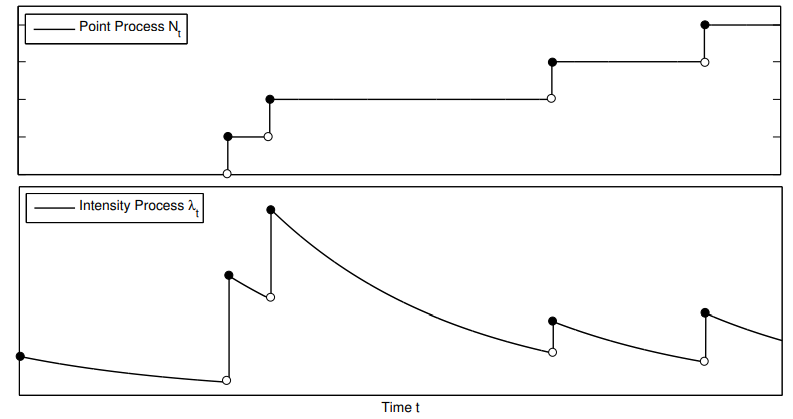
\includegraphics[width=0.75\textwidth]{hawkes.PNG}
\caption{Proceso de Hawkes.}
\label{f:f5}
\end{figure}

Por otro lado, este proceso de Hawkes ${N_t}_{t\geq0}$ puede ser construido alternativamente como un \textit{cluster} de Poisson en $\Re_{+}$ si los
\textit{clusters} siguen una estructura de ramificación. Esta definición es útil para aplicaciones en economía.

\textbf{Definición 2.2} Un proceso de Hawkes con \textit{rate} exponencialmente decreciente es un proceso de \textit{clusters} de Poisson 
$C=\left\{ (T_i,Y_i) \right\}_{i=1,2,\ldots}$ con tiempos $T_i\in\Re_{+}$ y procesos $Y_i$ tal que el número de puntos/procesos en $(0,t]$ viene 
definido por $N_t=N_{C(0,t]}$. Los centros de los \textit{clusters} son puntos a los que llamamos inmigrantes, el resto se llaman descendientes y tienen 
la siguiente estructura:
\begin{itemize}
    \item[\textbf{(a)}] Los inmigrantes $I={T_m}_{m=1,2,\ldots}$ en $\Re_{+}$ se distribuyen como un proceso no homogéneo de Poisson con \textit{rate}
    $a+(\lambda_0-a)e^{-\delta t}, t\geq0$
    \item[\textbf{(b)}] Los procesos ${Y_m}_{m=1,2, \ldots }$ asociados a inmigrantes $I$ son variables aleatorias independientes e idénticamente
    distribuidas con $Y_m\sim G$, por lo que son independientes a los inmigrantes.
    \item[\textbf{(c)}] Cada cluster $C_m$ es un conjunto aleatorio formado por generaciones del orden $n=0,1\ldots$ siguiendo la siguiente estructura de 
    ramificación:
    \begin{itemize}
        \item El inmigrante y su proceso $(T_m,Y_m)$ son la generación 0.
        \item Recursivamente, dadas las generaciones $n=0,1,\ldots$ en $C_m$, cada $(T_j,Y_j)\in C_m$ de generación $n$ genera un proceso de Poisson de
        descendencia $n+1$ en $(T_j,\infty)$ con intensidad $Y-je^{-\delta(t-T_j),t>T_j}$, donde $Y_j$ es independiente de las generaciones anteriores.
    \end{itemize}
    \item[(\textbf{d})] $C$ consiste en la unión de todos los clusters, es decir $C=\bigcup_{m=1,2,\ldots}C_m$.
\end{itemize}

Ambas definiciones son equivalentes. La condición estacionaria es $\delta>\mu_{1_G}$ donde $\mu_{1_G}=\int_{0}^{\infty}ydG(y)$

El el artículo nos dan también el valor medio y la varianza de $\lambda$, también nos dan el valor medio de $N_t$

\begin{align*}
    \mathcal{E}[\lambda_t|\lambda_0] =& \dfrac{a\delta}{\kappa}+\left( \lambda_0-\dfrac{a\delta}{\kappa} \right)e^{-\kappa t}\\
    \text{Var}[\lambda_t|\lambda_0] =&  \dfrac{\mu_{2_G}}{\kappa}\left[ \left( \dfrac{a\delta}{2\kappa} \right)e^{-2\kappa t} 
    \left( \lambda_0-\dfrac{a\delta}{\kappa} \right)e^{-\kappa t}+\dfrac{a\delta}{2\kappa}\right]
\end{align*}
donde $\kappa=\delta-\mu_{1_G}>0$, $\mu_{2_G}=\int_{0}^{\infty}y^2$, y el valor medio de $N_t$ 
$$\mathcal{E}[N_t|\lambda_0]=\dfrac{a\delta}{\kappa}t+\dfrac{1}{\kappa}\left( \lambda_0-\dfrac{a\delta}{\kappa} \right)(1-e^{-\kappa t}) $$

Un ejemplo dado la siguiente función el kernel:

$$g(y)=\beta e^{-\beta y}y,\beta>0$$
Por lo tanto, el primer y segundo momento son $\mu_{1_G}=\dfrac{1}{\beta}$ y $\mu_{2_G}=\dfrac{2}{\beta^2}$. Dados los siguientes parámetros 
$$(a,\delta;\beta;\lambda_0)=(0.9;1.0;1.2;0.9)$$
y tomando $T=t_{max}=100$ obtenemos los siguientes valores
\begin{figure}[H]
\centering
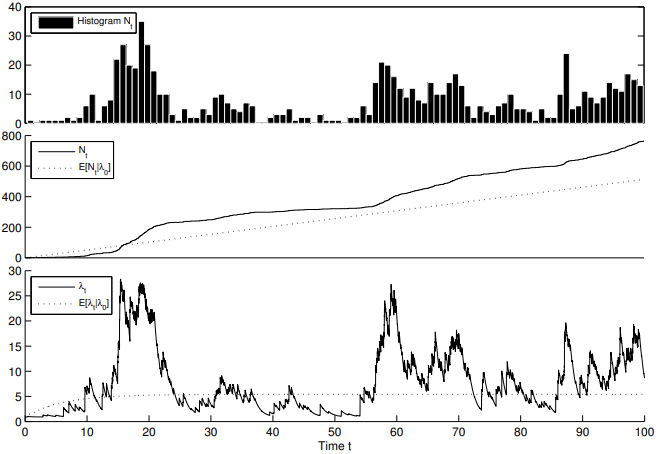
\includegraphics[width=0.75\textwidth]{Hawkes2.PNG}    
\end{figure}

La demostración matemática del algoritmo se basa en que dado el salto k-ésimo en el tiempo $T_k$, el proceso tiene una intensidad que sigue la ecuación:
$$\dfrac{d\lambda_t}{dt}=-\delta(\lambda_t-a)$$
con la condición inicial $\lambda_t|_{t=T_k}=\lambda_{T_k}$, cuya solución es:
$$\lambda_t=(\lambda_{T_k}-a)e^{-\delta(t-T_k)}+a,\qquad T_k\leq t< T_k+S_{k+1}$$
yla probabilidad acumulada del tiempo entre evéntos k+1-ésimo, $S_{k+1}$, es:
\begin{align*}
    F_{S_{k+1}}(s)= &P{S_{k+1}\leq s}\\
    =&1-P{S_{k+1}\leq s}\\
    =&1-P{N_{T_{k+s}-N_{T_k}}=0}\\
    =&1-exp \left( -\int_{T_k}^{T_{k+s}} \lambda_u du\right)\\
    =&1-exp \left( -\int_{0}^{s} \lambda_{T_{k+v}^+} dv\right)\\
    =&1-exp \left( -\left( \lambda_{T_k}^+-a \right) \dfrac{1-e^{-\delta s}}{\delta}-as \right)
\end{align*} 

Con el método de la transformada inversa podemos obtener:

$$S_{k+1}\overset{\mathcal{D}}{=}F^{-1}_{S_{k+1}}(U),\quad U\sim U[0,1]$$

De todas formas, podemos evitar invertir la función $F_{S_{k+1}}$ descomponiendo $S_{k+1}$ en dos variables aleatorias independientes más simples:

$$S_{k+1}\overset{\mathcal{D}}{=}S_{k+1}^1\wedge S_{k+1}^2$$,
donde 

\begin{align*}
    P\left\{ S_{k+1}^{(1)}>s \right\} =&exp \left( -\left( \lambda_{T_k^+}-a \right)\dfrac{1-e^{-\delta s}}{\delta} \right), \\
    P\left\{ S_{k+1}^{(2)}>s \right\} =& exp \left( -as \right)
\end{align*}
Ya que se cumple que:

\begin{align*}
    P\left\{ S_{k+1}>s \right\} =& exp\left(  -\left( \lambda_{T_k^+}-a \right)\dfrac{1-e^{-\delta s}}{\delta} \right)\times e^{-as}\\
    =& P\left\{ S_{k+1}^{(1)}>s \right\}\times P\left\{ S_{k+1}^{(2)}>s \right\}\\
    =& P\left\{ S_{k+1}^{(1)} \wedge S_{k+1}^{(2)}>s \right\}
\end{align*}

Por lo que para la simulación de $S_{k+1}^{(1)}$, debido a que se cumple:

$$F_{S_{k+1}^(1)}(s)=\left\{ S_{k+1}^{(1)}\leq \right\}=1-exp \left( -\left( \lambda_{T_k^+}-a \right)\dfrac{1-e^{-\delta s}}{\delta}  \right)$$
Podemos establecer que:

$$exp \left( -\left( \lambda_{T_k^+}-a \right)\dfrac{1-e^{-\delta s}}{\delta}  \right) \overset{\mathcal{D}}{=}U_1$$
que podemos invertir fácilmente como
$$S_{k+1}^{(1)}=-\dfrac{1}{\delta}ln\left( 1-\dfrac{\delta log(U_1)}{\lambda_{T_k^+}-a} \right)$$

Notar que $S_{k+1}^{(1)}$ es una variable aleatira defectuosa, lo que quiere decir que puede valer $\infty$ con probabilidad no nula. Es decir, 
$$T \text{es defectuosa si } P\left\{ T=\infty \right\}>0$$
en nuestro caso:

$$\lim_{s\to\infty}F_{S_{k+1}^{(1)}}(s)=P\left\{ S_{k+1}^{(1)}\leq \infty \right\}1-exp\left( -\dfrac{\lambda_{T_k^+}-a}{\delta} \right)<1   $$

y la condición para que la simulación sea válida es $S_{k+1}^{(1)}$ es que $D_{k+1}>0$ donde

$$D_{k+1}=:1+\dfrac{\delta lnU_1}{\lambda_{T_k^+}-a}$$

De forma similar, para la simulación de $S_{k+1}^{(2)}$, que se distribuye exponencialmente:

$$S_{k+1}^{(2)}\overset{\mathcal{D}}{=}-\dfrac{1}{a}lnU_2$$

Por lo tanto, para la simulación de $S_{k+1}$, podemos tomar:

$$
S_{k+1}\overset{\mathcal{D}}{=} 
\begin{cases}
    S_{k+1}^{(1)}\wedge S_{k+1}^{(2)} & \text{if } D_{k+1} >0\\
    S_{k+1}^{(2)} & \text{if } D_{k+1} \leq 0
\end{cases}
$$

Finalmente, el salto temporal k-ésimo, vendrá dado por: 
$$T_{k+1}=T_k+S_{k+1}$$
y los saltos en $\lambda$ y $N$

\begin{align*}
    \lambda_{T_{k+1}}=&\lambda_{T^-_{k+1}}+ \overbrace{(\lambda_{T_k}-a)e^{-\delta \overbrace{(T_{k+1}-T_k)}^{S_{k+1}}}+a}^{Y_{k+1}}\\
    N_{T_{k+1}}=&N_{T_k}+1
\end{align*}

\chapter{The Elements of Hawkes Processes}

\section{Teoría básica}
Antes de empezar a estudiar los procesos de Hawkes vamos a recordar algunos conceptos básicos. Primero daremos definiciones a procesos de cuenta y a procesos 
puntuales junto a su notación. Después veremos el concepto de función de intensidad condicionada y compensador, ambos esenciales para entender los procesos de Hawkes. 
\subsection{Procesos de cuenta y procesos puntuales}
Comenzamos con la definición de un proceso de cuenta.

\textbf{Definición 1}. Un proceso de cuenta es un proceso estocástico $(N(t))\,:\,t\geq 0$ tomando valores en $\mathbb{N}_0$ que cumple que $N(0)=0$, es finito y es una función escalón
creciente hacia la derecha con incrementos de tamaño $+1$. 

Denotaremos $(\mathcal{H}(u)\,:\,u\geq 0)$ la historia de las llegadas en el tiempo $u$. Estrictamente hablanco $\mathcal{H}(\cdot)$ es una filtración, que es una secuencia creciente de 
$\sigma$-álgebras.

Un proceso de cuenta puede verse como una cuenta cumulativa de llegadas al sistema en el tiempo actual. Otra forma de caracterizar estos procesos es considerar una secuencia de tiempos 
de llegadas aleatorio $\mathbf{T}=[T_1,T_2,\ldots]$ en los que el proceso de cuenta $N(\cdot)$ se ha producido.  





\end{document}